%%==================================================
%% diss.tex for SJTU Master Thesis
%% based on CASthesis
%% modified by wei.jianwen@gmail.com
%% version: 0.3a
%% Encoding: UTF-8
%% last update: Dec 5th, 2010
%%==================================================

% 字号选项: c5size 五号(默认) cs4size 小四
% 双面打印(注意字号设置)
%\documentclass[cs4size, a4paper, twoside]{sjtuthesis} 
% 单面打印(注意字号设置)
\documentclass[cs4size, a4paper, oneside, openany]{sjtuthesis} 

%\usepackage[]{algorithm2e}

% \usepackage[sectionbib]{chapterbib}%每章都用参考文献

\newboolean{DOIT}
\setboolean{DOIT}{false}%编译某些只想自己看的内容,编译true,否则false

%% 行距缩放因子(x倍字号)
\renewcommand{\baselinestretch}{1.3}

% 设置图形文件的搜索路径
\graphicspath{{figure/}{figures/}{logo/}{logos/}{graph/}{graphs}}

%%========================================
%% 在sjtuthesis.cls中定义的有用命令
%%========================================
% \cndash 中文破折号
% 数学常量
% \me 对数常数e
% \mi 虚数单位i
% \mj 虚数单位j
% \dif 直立的微分算符d为直立体。
% 可伸长的数学箭头、等号
% \myRightarrow{}{}
% \myLeftarrow{}{}
% \myBioarrow{}{}
% \myLongEqual{}{}
% 参考文献
% \upcite{} 上标引用
%%========================================


\begin{document}

%%%%%%%%%%%%%%%%%%%%%%%%%%%%%% 
%% 封面
%%%%%%%%%%%%%%%%%%%%%%%%%%%%%% 

% 中文封面内容(关注内容而不是形式)
\title{应用过完备稀疏字典技术的流体模拟}
\author{李\quad{}欢}
\advisor{杨旭波}
\degree{工程硕士专业}
\defenddate{2014年12月}
\school{上海交通大学}
\institute{软件学院}
\studentnumber{1120379074}
\major{软件工程}

% 英文封面内容(关注内容而不是表现形式)
\englishtitle{Fluid Simulation Using Overcomplete Dictionaries Based on Sparse Coding}
\englishauthor{\textsc{Huan Li}}
\englishadvisor{Prof. \textsc{Xubo Yang}}
\englishschool{Shanghai Jiao Tong University}
\englishinstitute{\textsc{School of Software Engineering} \\
  \textsc{Shanghai Jiao Tong University} \\
  \textsc{Shanghai, P.R.China}}
\englishdegree{Master Degree}
\englishmajor{Engineering}
\englishdate{December, 2014}

% 封面
\maketitle

% 英文封面
\makeenglishtitle

% 论文原创性声明和使用授权
\makeDeclareOriginal
\makeDeclareAuthorization

%%%%%%%%%%%%%%%%%%%%%%%%%%%%%% 
%% 前言
%%%%%%%%%%%%%%%%%%%%%%%%%%%%%% 
\frontmatter

% 摘要
%%==================================================
%% abstract.tex for SJTU Master Thesis
%% based on CASthesis
%% modified by wei.jianwen@gmail.com
%% version: 0.3a
%% Encoding: UTF-8
%% last update: Dec 5th, 2014
%%==================================================

\begin{abstract}

烟雾、流水等流体是自然环境的重要组成部分,计算机模拟的流体行为能增添虚拟现实的真实感。近年来,在计算机图形学领域,已经出现了一大批稳定、逼真、比较高效的流体动画模拟方法,并且大量地应用到了影视游戏等产业。但是,基于速度场的欧拉流体模拟方法在计算大规模的流体动画时,投影步骤需要耗费大量的计算时间,成为欧拉流体模拟方法的瓶颈。

针对欧拉流体模拟方法的投影步骤,本文提出一种应用过完备稀疏字典技术的流体模拟方法,从流体场数据的局部细微结构入手,利用稀疏编码技术,建立能够匹配并重构高精度空间的复杂流体数据稀疏表示的过完备稀疏字典。然后线性组合该高精度度字典与下采样矩阵生成适用于低精度流场数据的过完备稀疏字典。其下采样矩阵与下采样高精度速度场到其低精度空间版本的下采样矩阵是同一矩阵,故理论上该低精度空间的过完备字典能够匹配低精度速度场数据的稀疏表示。

同时,为了将超完备稀疏字典技术应用到流体的加速模拟中,本文还建立了一个适用于流体模拟的重构上采样框架。该框架在投影步骤之前将流体的高精度速度场数据下采样到低精度网格上,在低精度网格上计算投影步骤,再利用超完备稀疏字典技术,将低精度流体的速度场数据还原到其高精度版本,并将还原后的高精度流场数据用于下一帧的计算。该框架巧妙地将欧拉方法的瓶颈步骤放到了低精度网格上计算,有效地避开了投影步骤的高耗时问题,从整体上提高了流体模拟的计算效率。

本文提出的方法与框架理论上适用于所有的欧拉流体模拟方法,并且用户可以根据自己的需求选择合适的降采样矩阵降采样流体速度场数据,该方法与框架具有可快速移植的特点。

本文提出的方法适用于模拟速度较慢的流体模拟方法。实验部分给出了本文方法的实验效果图,实验结果表明,本文方法能在一定程度上恢复流场的细节。在选取合适的参数时,即使与模拟较快的流体模拟器相比,本文的方法也可以在一定程度上加快流体模拟的速度。

  \keywords{\large 流体动画,过完备稀疏字典,稀疏编码,重构上采样,投影}
\end{abstract}

\begin{englishabstract}

Smoke, water and other fluids is an important part of the natural environment, and the computer simulation for fluid behavior of real world can make the virtual world more real. In recent years, the fields of computer graphics have proposed a lot of stable, realistic, efficient fluid simulation method, and have been widely used in movie and video game industry. However,  when simulating large-scale fluid scene, the projection step of Euler method which based on the computation of velocity field will be very time-consuming, and it is the bottleneck of Euler method of fluid simulation. 

Considering the bottleneck of Euler method of fluid simulation, the paper proposed a method applies a couple of overcomplete dictionaries based on sparse coding into fluid simulation. We use the local fine structure of high-resolution fluid data to learn an overcomplete dictionary, which can match various complex local fine structures of high-resolution fluid data and be used to recover these local fine structures by combined with the sparse representation. We calculate a low-resolution dictionary by multiplying the learned high-resolution dictionary with a down-sampling matrix. The down-sampling matrix will also be used to down-sample the high-resolution fluid velocity data to its low-resolution version, thus in theory, this dictionary of low-resolution space can be used to decomposite the sparse representation of low-resolution velocity field.

Meanwhile, in order to accelerate the simulation of fluid animation by using overcomplete dictionaries, this paper also established a reconstruction and up-sampling framework for fluid animation. this paper also established a reconstruction and up-sampling framework for fluid animation, which maps the local fine structures of the high-resolution fluids data to their low-resolution version before the projection step, 
and the projection step is computed on a low-resolution grid, after which we use the trained overcomplete dictionaries to up-sample and reconstruct the low-resolution fluid data to their high-resolution version. This high-resolution fluid data will be used to compute velocity field of the next frame.  This framework
avoids to compute the projection step on a high-resolution grid, which can accelerate the computation of fluid simulation.

The method propsed by this paper can be applied to any fluid simulator based on Euler, and the down-sampling matrix can be customized on one's own purpose. this framework can be easily intergrated to any fluid simulators.

Our framework can be applied to the simulators which is computationally slow on a higher resolution grid and want to accelerate to a certain extent. The result of this method will be shown in the Result Section, and proves that our method can recover the details of fluid to a certain extend. Using the appropriate parameters, even compared with a relatively fast fluid simulator used in our experiment, our method can accelerate the computation speed to a certain extend.

  \englishkeywords{\large fluid animation, overcomplete dictionaries, sparse coding, reconstruct and up-sampling, projection}
\end{englishabstract}


% 目录
\tableofcontents
% 插图索引
\listoffigures
\addcontentsline{toc}{chapter}{\listfigurename} %将图索引加入全文目录
% 表格索引
\listoftables
\addcontentsline{toc}{chapter}{\listtablename}  %将表格索引加入全文目录

% 主要符号、缩略词对照表
%%==================================================
%% symbol.tex for SJTU Master Thesis
%% based on CASthesis
%% modified by wei.jianwen@gmail.com
%% version: 0.3a
%% Encoding: UTF-8
%% last update: Dec 5th, 2010
%%==================================================

\chapter{主要符号对照表}
\label{chap:symb}
\begin{tabular}{ll}

 \hspace{2em}${\boldsymbol u}$       & \hspace{5em}流体速度场 \\
 \hspace{2em}$p$ \qquad     & \hspace{5em}压强场 \\
 \hspace{2em}$\upsilon$       & \hspace{5em}粘性系数 \\
 \hspace{2em}$\rho$ \qquad     & \hspace{5em}密度 \\
 \hspace{2em}${\boldsymbol g}$ \qquad     & \hspace{5em}流体外力加速度 \\
 \hspace{2em}${\nabla \cdot \nabla}$ \qquad     & \hspace{5em}拉普拉斯算子 \\
 \hspace{2em}$\lambda$ \qquad     & \hspace{5em}拉格朗日算子 \\
 \hspace{2em}$\alpha$ \qquad    & \hspace{5em}稀疏表示系数 \\
 \hspace{2em}${\boldsymbol u}$       & \hspace{5em}高精度流体速度场 \\
 \hspace{2em}${\boldsymbol {\tilde u} }$ \qquad & \hspace{5em}低精度流体速度场\\
 \hspace{2em}${\boldsymbol D_h}$ \qquad     & \hspace{5em}密度 \\
 \hspace{2em}${\boldsymbol D_l}$ \qquad     & \hspace{5em}拉格朗日算子 \\
 \hspace{2em}${\boldsymbol S}$ \qquad    & \hspace{5em}降采样矩阵 \\

\end{tabular}


%%%%%%%%%%%%%%%%%%%%%%%%%%%%%% 
%% 正文
%%%%%%%%%%%%%%%%%%%%%%%%%%%%%% 
\mainmatter


%% 各章正文内容
%%==========================
%% chapter01.tex for SJTU Master Thesis
%% based on CASthesis
%% modified by wei.jianwen@gmail.com
%% version: 0.3a
%% Encoding: UTF-8
%% last update: Dec 5th, 2010
%%==================================================

%\bibliographystyle{sjtu2} %[此处用于每章都生产参考文献]
\chapter{绪论}
\label{chap:background}

\section{研究背景}

烟雾、流水等流体是自然界环境的重要组成部分,计算机模拟的流体行为能增添虚拟现实的真实感,更好地烘托环境气氛。在传统的动画开发环境下,流体动画的每一帧为动画师手工绘制,虽然这样能灵活可控地进行创作,但所需工作量巨大,而且难以获得高精度效果。随着流体动画技术和相关应用需求的发展,流体动画采用计算机模拟和渲染流体现象,是 计算机图形学领域的一个非常重要的研究分支,在影视游戏、虚拟现实、科学计算等领域有广泛的应用价值。

在计算机图形学领域,近年来出现了一大批稳定、逼真、比较高效的流体模拟方法,并且已经大量地应用到了影视游戏等产业,在电影设计的辅助下,成功地模拟出了海浪奔涌、水珠迸溅、烟雾缭绕等震撼人心的效果。

但是,随着虚拟现实和数字媒体应用的发展,具有复杂流体动态效果的大规模流体动画将扮演日益重要的角色,而现有的流体模拟方法都受限于对大规模场景的海量动画数据的采样和计算,导致在计算较大规模的流体动画的每一帧时,需要消耗几十甚至几小时的时间。因此,研究大规模流体动画的快速高效模拟方法具有重要的应用意义。现有研究中,人们提出了很多方法改进流体模拟的速度,但是仍然存在很多问题。有些方法通过简化流体力学模型达到加速的目的,但其计算耗费仍然非常巨大。

压缩感知颠覆了经典的Nyquist定理,被誉为学术界的一个“Big Idea''。该定理在2006年诞生后的短短几年里,就很快在通信、声音、图像等领域成功应用,并取得了令人难以置信的突破。基于压缩感知理论的超完备稀疏字典技术指出,如果训练字典足够完备,就可以利用重构上采样方法准确地重构出原信号数据。近年来,超完备稀疏字典也已在图形处理、信号处理、分类等领域得到了成功应用。本课题拟针对大规模流体动画的快速高效模拟问题,探索将压缩感知理论技术应用到流体动画领域的方法与框架。

\section{国内外研究现状}
\subsection{流体模拟的基本方法}
\label{sec:basicMethod}
 计算机动画领域中的流体动画模拟方法,不同于传统工程计算中的计算流体力学追求高精度的数值计算,而是更加看重视觉效果和计算效率,故计算机动画中使用的流体动画模拟算法具有高效、简单和易于实现等特点。基于物理的流体动画方法通过求解Navier-Stokes物理方程组来模拟流体,主要有三种基本模拟方法:拉格朗日粒子法,欧拉网格法和基于旋度的方法。
 
 \subsubsection{欧拉方法}
\label{sec:Euler}

欧拉法通过在空间中设置固定的点,观测流体的物理量(如速度、密度、温度等)在通过该点时随着时间的变化来表示流体的运动。通常在欧拉方法中,流体空间被划分成规则或不规则的网格,通过在这些离散网格上求解Navier-Stokes方程组得到一定时间序列中这些离散网格上的物理量的变化过程,从而达到描述流体运动的目的。1997年Foster和Metaxas~\cite{foster1997modeling}建立一种气体在热气浮力作用下运动的气体运动模型,率先把流体模拟引入进算计图形学领域。1999年stam~\cite{stam1999stable}首次定义了一种投影的方法,将流体模拟的基础模型分解为四个主要部分分别求解,同时还引入了一种无条件稳定的半拉格朗日方法,奠定了欧拉法的基础。Fedkiw等人~\cite{fedkiw2001visual}在2001年提出的对烟模拟的框架,基本完善了欧拉法的步骤和流程;Enright等人~\cite{enright2002animation}在2002年提出了对复杂流体表面模拟的框架,至此,采用欧拉模拟流体的框架也基本稳定。

 \subsubsection{拉格朗日粒子法}
\label{sec:Lagrangian}

拉格朗日粒子法将流体当做一个粒子系统来处理。模拟区域中的流体或者固体点都相应地标记成一个独立具有速度和位置属性的粒子,通过描述这些粒子在受到外力和周围其他粒子互相影响之后在一定时间序列内的物理量变化来描述流体运动。M{\"u}ller,Adams~\cite{muller2003particle}~\cite{adams2007adaptively}等人采用了该方法模拟流体。拉格朗日方法具有计算量小,模拟速度快的优点,但是难以保持无散条件,并且难以从大量离散的粒子中提取出光滑液体表面用于渲染,不适合需要照片级真实感的场合。

 \subsubsection{基于旋度的方法}
\label{sec:Vortex}

基于旋度的方法通过描述涡旋粒子随着时间的的运动来模拟流体动画的效果。该类方法通过计算涡旋粒子的旋度变化来计算流体的速度变化,而流体的细节主要来自于涡旋粒子,故该方法可以生成较多的细节。但是难以处理各种边界条件,如自由表面和固体边界等,且难以保证模拟的稳定性。Alexis~\cite{angelidis2005simulation}~\cite{angelidis2006controllable}等人分别在2005年和2006年提出了基于Vortex Filament的基于旋度的流体模拟方法,并且成功地生成了烟雾缭绕的效果。

\subsection{流体模拟优化方法}
\label{sec:optimization}
相较于其他方法,欧拉法因易于离散和求解无散条件等优点,相关的研究工作最多。但是欧拉方法的模拟效果依赖于网格精度,想要模拟出涡旋等细节,需要使用足够高的网格精度才能实现。但是提高网格的精度会大幅度地增加模拟的时间开销,常常会消耗几个甚至几十个小时来计算很小一段时间帧的流体动画。在学术界,拟针对如果提高流体模拟的速度,提出了各种优化方法,主要相关工作可归纳为四类。

\subsubsection{自适应网格方法}
\label{sec:adaptive-gird}

在流体模拟过程中,并不是所有的模拟区域都包含有丰富的细节特征。自适应采样方法针对流场的不同级别的细节特征,分配不同粗细的网格,对细节丰富的高频流场区域,分配最细的网格,而对变化平缓的低频流场区域,则分配较细的网格。如八叉树方法~\cite{losasso2004simulating},对空间进行自适应的八叉树划分,在边界等重要细节区域划分出更精细网格,而将非重要区域划分为粗略网格。该类方法的优点是能在保持细节质量的同时,降低总体采样数量。但是由于要控制不同级别的网格精度,也使得算法的数据处理计算更为复杂。

\subsubsection{混合模型方法}
\label{sec:mix-model}

该类方法的基本思想是根据流场不同区域的计算要求,分别采用不同类型的计算模型。现有的该类方法有混合网格法~\cite{dobashi2008fast}、网格-粒子混合法~\cite{zhu2010creating}、欧拉-旋度混合法~\cite{golas2012large}等等。这类方法结合了不同模型的优点,可在优化计算速度的同时,保留流体动画尽可能多的细节。如文献~\cite{dobashi2008fast}全局采用粗略的网格,局部采用细致的网格以捕捉细节;文献~\cite{zhu2010creating}利用粒子进行对流,借助网格解压力项与无散条件;文献~\cite{golas2012large}采用欧拉网格处理自由边界和障碍物边界等边界条件,可以有效地避开基于旋度方法不能处理边界条件的缺陷,在其他无边界区域采用基于旋度的方法,充分地利用了基于旋度的方法模拟速度快的优点。但是这类方法需要维护不同不同计算模型及其之间的数据耦合,增加了算法设计和实现的难度,耦合过程中也会带来额外的精度损失。

\subsubsection{低-高精度重采样方法}
\label{sec:low-high-resampling}

欧拉方法通常分成三个步骤:对流、添加外力和投影。当提高网格精度时,计算投影步骤所消耗的时间会以指数级增长,成为该方法所有步骤中耗时最为显著的一个部分。低-高精度重采样方法的基本思想就是尽量减少投影步骤的计算时间,其具体做法为将高耗时的投影步骤放到低精度场计算。Yoon等人~\cite{yoon2009procedural}提和Kim等人~\cite{kim2008wavelet}提出一种过程化合成方法,先计算一个低精度流场,将低精度流场线性上采样,得到高精度流场,再使用涡粒子或者小波湍流合成高精度流场细节。M.Lentine ~\cite{lentine2010novel}等人采用高精度网格对液体表面追踪,通过液体无偏差滤波器将获得的高精度表面降采样到低精度网格,求解低精度下的泊松方程,保证无散条件,再将低精度的速度场映射回高精度网格,然后在每个粗网格内进行一次局部高精度网格的泊松方程求解,以保证高精度下速度场的无散条件,整体提高了高精度网格上的泊松方程求解效率。但是这类方法目前还缺乏高效准确的重采样理论和方法支持。

\subsubsection{模型缩减法}
\label{sec:ModelReduction}

该方法通过对流体数据和计算模型进行大幅缩减,达到实时模拟的目的。Andrie~\cite{treuille2006model}提出的模型缩减方法,针对一个给定场景,先用离线的高精度模拟器,预计算一组高精度流体模拟的结果,利用其得到一组代表流场特征的正交基函数,将流体速度场缩减变换到一个小的基函数空间中,然后在缩减模型中求解方程。由于其缩减后的变量个数不依赖于空间精度,故可大幅提升运算效率。但是其代价是大幅降低了模型准确度,并且不能灵活变换场景。~\cite{wicke2009modular}利用模块化思想加以改进,对场景分块计算,每个分块分别采用模型缩减的方法进行模拟,但是这种方法只适合于像拼版游戏对场景做少量重组变化,场景普适性差。

\subsection{过完备稀疏字典技术}
\label{sec:overcompleteDictionaries}

压缩感知是2006年由Donoho,Candes和Tao等数学家建立起来的一个严格的数学理论~\cite{candes2006near}~\cite{donoho2006compressed}~\cite{candes2008introduction},该定理在诞生后的短短几年里,就很快在通信、声音、图像等领域成功应用,并取得了令人难以置信的突破。~\cite{kroeker2009face}结合稀疏编码技术和压缩感知理论,成功地识别出完全被噪声遮蔽,连人眼都无法辨认的图像。近年来,基于压缩感知技术的过完备字典技术也成为了一个热门话题,

数据的稀疏表示模型假设信号可以由一个预定义字典中的很少量原子的线性组合表示,因此选择一个使信号稀疏化的字典是一个极其重要的问 题。R. Rubinstein~\cite{rubinstein2010dictionaries}描述了选择字典的两种方法: (1)基于数据的数学模型建立一个稀疏字典;(2) 使用训练数据集学习一个训练字典。第一种方法基于谐波分析,对一个更简单的数学运算建模,并根 据该模型设计一个高效表示。如傅里叶字典根据平滑函数建模,小波字典根据含奇异点的分段平滑函 数建模。该类字典具有不涉及字典矩阵乘法,快速隐实现的特点,但是相较于自然现象的复杂性,该类模型过于简单化。第二种方法假设复杂自然现象的结构可以从数据本身更直接地提取,这种直接提取的好处是可以更好地适应特定数据。近年来基于训练数据集的字典方法受到稀疏表示理论影响,都集中于研究\(l^0\)和\(l^1\)稀疏,使得方法得以简化并应用最新的稀疏编码技术。

疏密重构上采样方法,通过求解Lasso问题,得到输入信号的稀疏表示,然后将该信号的稀疏表示与训练字典线性组合,推断出输入信号的重构上采样信号。该方法的重构效果与方法依赖于过完备训练字典,不同的训练字典,需采用不同的重构上采样方法。Yang等人~\cite{yang2010image}~\cite{yang2008image}~\cite{yang2012coupled}将压缩感知技术应用到图像重构领域,达到了令人瞩目的效果;~\cite{marwah2013compressive}采用类似的方法,将压缩感知技术应用到照相机的光场重构,也取得了较为理想的效果。目前,在流体动画领域还没有任何使用感所感知技术的相关文献。

过完备稀疏字典技术融合训练字典和分析字典的优点,利用细数编码技术学习特定的训练数据,建立一个可以使训练数据足够稀疏化的字典。由于该字典拥有比原数据信号更多维度的基信号原子,故我们称该字典使过完备的。过完备字典技术指出,一个信号在其表示域可以表述成多种形式,能否选取最合适的表示取决于使用的字典和解码方法。1993年,~\cite{mallat1993matching}提出了一种基于冗余函数字典的新奇的分解方案;两年后,Chen, Donoho和Saunders发表了一篇基于basis pursuit分解的论文~\cite{chen1998atomic},他们的工作奠定了使用字典的稀疏信号表示方法的基础。多年来,正交和双正交的字典表示方法因其简单性和有效性在信号处理领域被广泛应用,如小波去噪~\cite{donoho1995noising}.但是该类型的字典方法受限于其表征能力,于是产生了过完备字典技术的发展。

\section{本文的主要工作及创新点}
\label{sec:creation}

实际上,自然界的流体现象可以看作是由很多局部细微结构组成的,因此,可以尝试将复杂流体数据用局部细微结构的线性组合来表示,这些局部细微结构可以从大量流体数据中采集、提取和存储,形成一个经验数据集,然后利用压缩感知理论中的稀疏逼近手段,将各种复杂流体数据转化为流体局部细微结构的稀疏表示。目前,流体领域还没有相关方法的文献出现,但是,在图像、音频与视频信号处理等领域,已经出现了大批相关的技术。本文借鉴流体模拟的过程化合成方法,将流体模拟中最为耗时的投影步骤放到低精度网格模拟,在较少的计算耗费下提供较多的流体模拟细节。然后使用基于稀疏编码的超完备字典技术,将低精度网格流场数 据重构上采样到高精度网格空间,用于下一帧模拟计算。

\subsection{主要研究工作}

基于压缩感知理论,本文尝试将应用在图像信号处理领域中的基于稀疏表示的过完备训练字典技术应用到流体动画领域,达到快速高效地模拟大规模流体动画的目的。

本文的主要研究工作包括如下部分:
\begin{itemize}
\item 学习复杂流体数据的稀疏表示和疏密样本映射,生成过完备的训练字典。实际上,自然界的流体现象可以看作是由许多局部细微结构组成的,因此可以尝试将复杂流体数据用局部细微结构的线性组合来表示,这些局部细微结构可以从大量流体数据中采集、提取和存储,形成一个经验数据集。如果这样的一个经验数据集可以表示几乎所有的流体现象的局部细微结构,我们称其为过完备的训练字典;
\item 流体疏密数据映射重构方法。利用压缩感知理论中的稀疏逼近手段,探索一个适合复杂流体疏密数据的重构方法;
\item 2D场景流体动画压缩采样的高效计算框架。借鉴已有的低-高精度重采样方法,在高精度流场上计算对流和加外力步骤,然后将高精度流场数据降采样投影到低精度网格计算投影步骤,保证无散条件,再使用过完备字典,将低精度流场数据重构到高精度流场中;
\item 解决疏密映射重构方法到流体模拟中导致的流体形态改变、边界条件问题。
\end{itemize}

\subsection{本文创新点}

目前,基于物理的计算机流体模拟技术已经较为成熟,但是如何快速地模拟流体动画而尽可能多且真实地保留住流体动画的细节,一直是一个研究的热点问题。本课题拟针对这样一个问题,探索压缩感知理论在流体动画领域的适用性,对流体动画领域有重要的意义。

本课题研究内容十分新颖,主要包括如下创新点:
\begin{itemize}
\item 将压缩感知理论引入流体动画研究领域,学习复杂流体细微结构,探索基于稀疏表示的过完备字典训练技术在流体动画领域的应用;
\item 通过线性组合高精度训练字典与一个下采样矩阵,计算生成能够表示低精度速度场空间的字典,并根据该低精度空间的字典获得低精度速度场的稀疏表示形式;
\item 基于压缩感知理论,系统地探索复杂流体数据的稀疏表示形式,建立基于局部细微结构的稀疏表示形式,提出适用于流体动画重构上采样的方法与框架。
\end{itemize}

\section{本文组织结构}
\label{sec:orgnization}

本文共有六个章节,第一章绪论部分主要介绍了本课题的研究背景与国内外现状,后面的五个章节依次为:

第二章主要介绍流体模拟部分的基础知识,主要包括流体模拟方法的一般方法和基本框架。该章节将会对基于网格的流体模拟方法做一个全面的介绍,并详细阐述流体模拟的基本数学模型——Navier-Stokes方程组。

第三个章节主要介绍基于稀疏编码的过完备稀疏字典方法的基础知识。该部分将会详细描述基于稀疏编码技术的双字典技术以及其重构框架。

在第四章节中,我们将会给出本文流体模拟方法的基本框架以及基于过完备稀疏训练字典的训练与在流体动画中的具体应用过程。

在第五章节中,我们将会给出大量的实验结果,探讨本文提出方法的可行性。我们会先给出本文提出方法在图像域的实验结果,证明本文提出的重构算法在实际应用中确实能够重构出额外的细节之后,再将本文的重构算法应用到流体模拟领域,并与双三次插值的重构结果相比较,证明本文提出的算法确实能在一定程度上增加流体的细节。

最后一个章节将会对本文的工作做一个总结,分析本文方法的局限性以及未来可能的研究方向。


%%==================================================
%% chapter02.tex for SJTU Master Thesis
%% based on CASthesis
%% modified by wei.jianwen@gmail.com
%% Encoding: UTF-8
%%==================================================

\chapter{流体模拟的基本方法与过完备训练字典技术}
\label{chap:fluidSimulation}

本文研究的内容是一个交叉性课题,主要包括应用重构上采样方法的流体动画计算框架和应用过完备稀疏字典技术的重构上采样方法。在介绍本文研究的流体动画计算框架和过完备稀疏字典方法之前,本章先介绍流体模拟的基本数学模型Navier-Stokes方程组和该模型求解的基本方法,并指出过完备稀疏字典技术重点研究的两个问题。

\section{Navier-Stokes方程组}
\label{sec:navier-stokes}

计算机图形学最有趣的问题之一是类流体行为的仿真,并且,不同的领域,对流体模拟求解的目标要求也有所不同。在特效产业中,模拟流体动画的目的是如何产生令人信服的譬如烟雾、水和火等流体的外观和行为;在计算机动画领域模拟流体动画,我们更关心的则是动画的视觉效果,而不是求解的准确性。尤其对于烟的模拟而言,我们更关心烟动画中的小规模细节,而不是速度场的数值精度。在基于仿真的流体模拟领域,流体力学被作为标准数学框架在使用。科学家们一致表示,Navier-Stokes方程式是模拟流体流动现象的一个很好的数学模型。

\subsection{Navier-Stokes方程组的描述形式}

在流体力学中,Navier-Stokes方程组描述了满足不可压条件的粘性流体,被称为世界上“最复杂的方程之一”。Navier-Stokes方程组的名字记录了推导出该方程组的人的姓名,分别是Claude Louis Navier 和 George Gabriel Stokes,通常也被简称为N-S方程组。可以写成如下形式~\cite{bridson2007fluid}:
\begin{equation}
\label{basicEq}
 \frac{\partial \boldsymbol u}{\partial t} + {\boldsymbol u} \cdot \nabla {\boldsymbol u} + \frac{1}{\rho} \nabla p= {\boldsymbol g} + \nu \nabla \cdot \nabla {\boldsymbol u}
\end{equation}
\begin{equation}
\label{imcompressible}
 \nabla \cdot {\boldsymbol u} = 0
\end{equation}

其中,\(\boldsymbol u\)表示流体的速度场。在欧拉网格方法中,该速度表示流体经过每个固定的点空间时所具有的速度矢量。在3D情况下,\(\boldsymbol u\)通常被写成\((u,v,w)\)的形式,分别表示3D空间标准坐标系下的\(\boldsymbol{x}, \boldsymbol{y}, \boldsymbol{z}\)三个方向上的速度大小。
 
\(p\) 表示压强场,在流体的内部,每个欧拉网格的中心都有存储了一个压强分量。

\(t\)代表时间。
 
\(\nu\)代表流体的粘性系数,\(\nu\)越大,表示流体的粘性越大。
 
\(\rho\)表示流体的密度。
  
 \(\boldsymbol g\)表示施加在流体上的外力合力产生的加速度,这些外力包括重力、浮力等。大部分情况下,流体只受重力的影响,故在此处,我们使用通常表示重力加速度的变量\(\boldsymbol g\)表示流体所受到的外力合力加速度。
 
 \(\nabla\)是向量空间的偏导数, 如\(\nabla {\boldsymbol u}\)表示速度场的偏导数。\(\nabla\) = (\(\frac{\partial}{\partial x}, \frac{\partial}{\partial y})\)表示2D空间的偏导,\(\nabla\) = (\(\frac{\partial}{\partial x}, \frac{\partial}{\partial y}, \frac{\partial}{\partial z})\) 则表示3D空间的偏导。另外,\(\nabla \cdot \nabla\)表示拉普拉斯算子。

\subsection{Navier-Stokes方程组的意义}
\label{sec:eqmeaning}

Navier-Stokes方程组对流体做了以下几个假设:第一,流体是连续的,该假设指液体的内部不能包含空隙,如雾状粒子的聚合、溶解的气泡等。第二,所有涉及到的场都是可微的,如压强场、速度场、密度场和温度场等。

Navier-Stokes方程组的式~\ref{basicEq}根据质量、动量和能量守恒的基本原理导出。我们可以把流体想象成一个粒子系统,每个粒子代表一个小水珠。那么,我们可以描述每个粒子的质量为\(m\),速度为\(\boldsymbol u\),体积为\(V\)。那么根据动量守恒定理,我们可以得到如下方程式:
\begin{equation}
\label{momentum}
 {\boldsymbol F} = m\frac{D{\boldsymbol u}}{D{t}}
\end{equation}

假设粒子受到的来自流体系统以外的力只有重力,表示为\(m{\boldsymbol g}\)。那么我们只需要分析流体粒子来自于粒子系统中其他粒子的力。

\begin{figure}[ht]
  \centering
   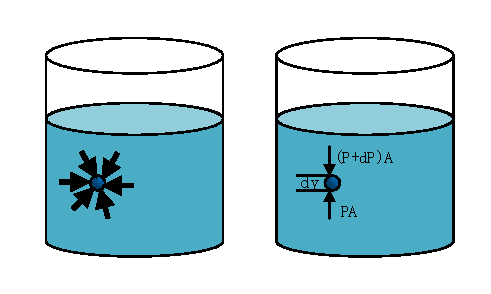
\includegraphics[height=1.8 in]{chap2/pressuredepth}
  \bicaption[pressuredepth]{}{流体粒子受压力示意图}{Fig}{Illustration of how fluid particles are affected by pressure}
\end{figure}

首先是压力。流体在运动的过程中,压力的作用会把高压区的流体推向低压区,从而使得流体粒子在整体上始终保持均匀分布的趋势。图\ref{pressuredepth}画出了流场内部流体粒子受到的所有压力的示意图。从左边的图中,我们可以看出流体粒子所受的压力来自四面八方。我们假设粒子每个方向上所受的压力都相等,根据图\ref{pressuredepth}右边的示例图片,可知流体粒子的压力只与其深度有关。为了简化模型,我们用压强梯度的负值\(-\nabla p\)表示压强的不平衡效果,而\(({-\nabla p})V\)表示粒子所有到的压力。

然后是粘滞力。粘滞力总是阻碍两个粒子之间的相对运动,并且相对运动越大,粘滞力越大。这里,我们直接给出粘滞力的表达式为\(V\mu{\nabla \cdot \nabla {\boldsymbol u}}\)。其中,\(\mu\)为动态粘性系数,是流体自身的属性,通常是常量。故用重力、压力以及粘滞力表示方程式~\ref{momentum}中的外力\(\boldsymbol F\),可得到流体运动的加速度方程:
\begin{equation}
 m\frac{D{\boldsymbol u}}{D{t}} = m{\boldsymbol g} - V{\nabla p} + V{\mu}{\nabla \cdot \nabla {\boldsymbol u}}
\end{equation}

我们已知\(\frac{V}{m} = \frac{1}{\rho}\),设变量\(\nu = \frac{\mu}{\rho}\),上述方程式两边都除以粒子的质量m,则有:
\begin{equation}
 \frac{D{\boldsymbol u}}{D{t}} = {\boldsymbol g} - \frac{1}{\rho}{\nabla p} + {\nu}{\nabla \cdot \nabla {\boldsymbol u}}
\end{equation}

展开速度场\(\boldsymbol u\)关于时间\(t\)的导数,即可得到方程式~\ref{basicEq}。

\begin{figure}[ht]
  \centering
   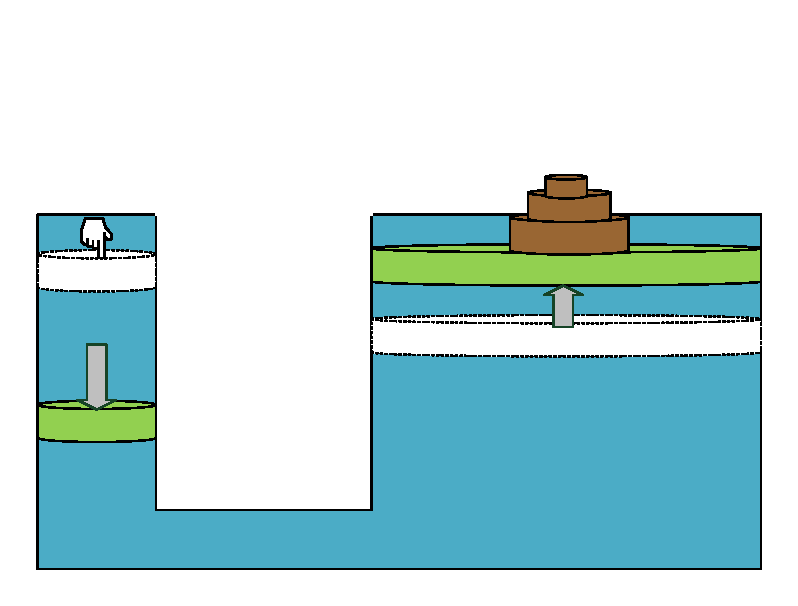
\includegraphics[height=2.3 in]{chap2/imcompressible}
  \bicaption[fig:imcompressible]{}{流体不可压示意图}{Fig}{Illustration of imcompressible condition}
\end{figure}

方程式~\ref{imcompressible}表示流体的不可压缩条件,而图~\ref{fig:imcompressible}展示了流体不可压缩时的宏观表现,即压缩流体时,流体会保持其体积不变。从微观的角度讲,当我们说流体是不可压缩的时,指的是在微观时间段\(\Delta t\)内,流入与流出流体任意体积为\(\Omega\)的流体表面的体积是相等的,即流体的体积变化速率为0,可以表示成如下形式:
\begin{equation}
{\iint_{\partial \Omega}}{\boldsymbol u} \cdot {\hat n} = 0 
\end{equation}

根据微积分基本定理,我们可以将上式转化为如下形式:
\begin{equation}
{\iiint_{\Omega}} \nabla \cdot {\boldsymbol u} = 0 
\end{equation}

由于上述方程式对于流体内部的任意体积\(\Omega\)都是成立的,故只有当被积函数处处为0时,上述函数积分才能为0。当上述积分方程式的被积函数为0时,即可得方程式~\ref{imcompressible}。

\subsection{忽略粘性力作用}

通常,在计算机动画模拟的数值计算中,会忽略掉粘性力这一项。因为相比较于其他作用力,粘性力的值通常是很小的。另外,在流体模拟的数值计算的过程中不可避免地会有数值耗散,而该数值耗散项的值的数量级与粘性力项的值的数量级比较接近,故可以近似认为数值耗散项替代了粘性力项的计算。并且从方程式~\ref{basicEq}中,我们可以看出,粘性力项的计算开销也比较大,忽略粘性力作用可以在很大程度上减少计算的开销。故流体模拟的一般方法求解的是如下形式的Navier-Stokes方程组:
\begin{equation}
\label{basicEqignoreVis}
 \frac{\partial \boldsymbol u}{\partial t} + {\boldsymbol u} \cdot \nabla {\boldsymbol u} + \frac{1}{\rho} \nabla p= {\boldsymbol g}
\end{equation}

\section{流体模拟的基本方法}

根据绪论部分的介绍,可知目前主要的流体模拟方法主要有三大类,即欧拉网格法、拉格朗日粒子法和基于旋度的方法。本文主要研究基于欧拉网格方法的重构上采样框架在流体动画领域的应用,故本章的该部分将会简单介绍用欧拉网格方法求解Navier-Stokes方程组的基本框架。

\subsection{网格介绍}

\begin{figure}
  \centering
   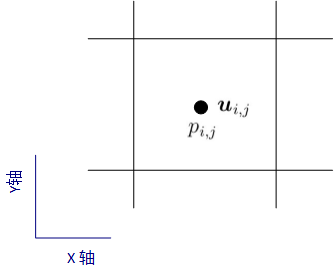
\includegraphics[height=1.6 in]{chap2/centergrid2D}
  \bicaption[fig:centergrid2d]{}{中心网格2D示意图}{Fig}{cells from 2D center grid}
\end{figure}

\begin{figure}[ht]
  \centering
   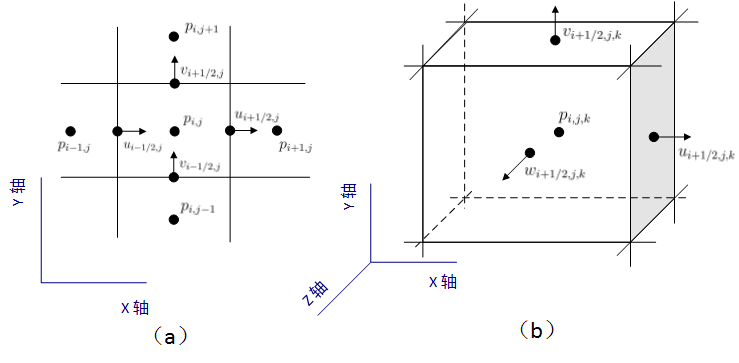
\includegraphics[height=2.5 in]{chap2/macgrid}
  \bicaption[fig:macgrid]{MAC网格示意图}{(a) 2D MAC网格示意图;(b) 3D MAC网格示意图}{Fig}{(a) one cell from the 2D MAC grid;(b) one cell from the 3D MAC grid}
\end{figure}

用欧拉方法求解流体动画时,需要对速度场离散化求解,即在网格上对其进行求解计算。最简单的网格模型是中心网格模型,该网格模型把所有的变量都存储在网格的中心点上,如图~\ref{fig:centergrid2d}描述了中心网格在2D场景下变量的存储方式,其中,$\boldsymbol u_{i,j}$表示位置为$(i,j)$处的网格点的速度场矢量,$p_{i,j}$表示同一网格位置的压强场。但是被更为广泛使用的是MAC网格模型,由Harlow等人~\cite{harlow1965numerical}提出。MAC网格实际上是一个交错的网格,变量存储在网格的不同位置上,并且存储在不同位置的变量有不同的含义,如图~\ref{fig:macgrid}所示,(a)和(b)分别描述了2D场景和3D场景下MAC网格各变量的存储方式,其中\(p\)是压力值,\(u,v,w\)分别表示速度场的三个分量。相较于中心网格,MAC网格的计算效率更高,并且更加稳定,故在欧拉网格方法中使用更为广泛。本文提出的流体模拟重构框架既适用于中心网格,也适用于MAC网格。

\subsection{欧拉网格方法及其计算框架}

Navier-Stokes方程组方程组虽然看起来简单,但是因为方程式~\ref{basicEqignoreVis}存在非线性项,故直接求解非常困难。为了简化求解过程,通常会把Navier-Stokes方程组分解成三个部分求解,分别为对流、体积力和压力/不可压缩部分。分别列出如下:
\begin{equation}
\label{eq:advection}
\frac{\partial {\boldsymbol u}}{\partial t} + {\boldsymbol u} \cdot \nabla {\boldsymbol u} = 0  \ \ \ \ \ (advection)
\end{equation}
\begin{equation}
\label{eq:addForce}
\frac{\partial {\boldsymbol u}}{\partial t} = {\boldsymbol g}  \ \ \ \ \ \ (body forces)
\end{equation}
\begin{equation}
\label{eq:projection}
\frac{\partial {\boldsymbol u}}{\partial t} + \frac{1}{\rho} \nabla p= 0 
\ \ \ \ \ 
 s.t. \ \ \ \ \ 
 \nabla \cdot {\boldsymbol u} = 0 \ \ \ \ \ \ (pressure/incompressibility)
\end{equation}

上述三个方程式通常对应欧拉方法的三个步骤,即式~\ref{eq:advection}对应对流步,通常表示为advection,该步骤把速度场\({\boldsymbol u}\)对流一个时间间隔\(\Delta t\);式~\ref{eq:addForce}对应外力步,表示成addForce,表示外力合力作用对流体速度场的加速度;式~\ref{eq:projection}对应投影步,表示为projection,该步骤保证前两步计算得出的速度场\({\boldsymbol u}\)是无散的,同时还保证流体速度场满足固体边界条件。

在这三个部分中,我们需要保证对流是在无散速度场中进行的,故advection步骤的运行需要以projection步骤的输出为前提。综上所述,可以归纳出欧拉网格方法的基本运算步骤如算法~\ref{Eulerframework}所示。

\begin{algorithm}%[htb]
\caption{ 流体模拟的基本框架伪代码.}
\label{Eulerframework}
\begin{algorithmic}[1] %这个1 表示每一行都显示数字
%\REQUIRE ~~\\ %算法的输入参数:Input
%coupled dictionaried $\boldsymbol D_l \ and \ \boldsymbol D_h$, low-resolution fluid velocity field $\bar {\boldsymbol u}$.
%\ENSURE ~~\\ %算法的输出:Output
%high-resolution fluid velocity field $\boldsymbol U$. 
  \STATE initialize a divergence-free velocity field ${\boldsymbol u}^{(0)}$;
\FOR{ every time step  $n = 0, 1, 2, ...$} 
    \STATE Do the advection: ${\boldsymbol u}^{A} = advection({\boldsymbol u}^n, \Delta t)$.
    \STATE  Do the addForce: ${\boldsymbol u}^{B} = {\boldsymbol u}^{A} + {\Delta t} {\boldsymbol g}$. 
    \STATE Do the projection: ${\boldsymbol u}^{n + 1} = projection({\Delta t}, {\boldsymbol u}^{B})$.
\ENDFOR
\end{algorithmic}
\end{algorithm}

根据Navier-Stokes方程组的三个分解方程式,可以看出流体模拟的三个步骤中,最为耗时的是投影步骤。该步骤实际上求解的是一个泊松方程,Stam~\cite{stam2003real}使用了经典的高斯赛德尔迭代方法求解,Foster 等人~\cite{foster2001practical}采用了预处理共轭梯度法(ICPCG)求解,ICPCG 因其优秀的性能,成为了求解投影步骤的主流。但是投影步骤仍然是流体模拟方法的瓶颈步骤。

在Stam~\cite{stam1999stable}提出了允许大时间步长的无条件稳定的半拉格朗日方法求解对流步骤之后,很多人针对如何提高对流步骤数值解的精度提出了一些改进方案,如MacCormack~\cite{selle2008unconditionally},BFECC~\cite{kim2005flowfixer}~\cite{dupont2003back},QUICK~\cite{molemaker2008low}等对流方法。这些对流方法在一定程度上丰富了流体动画的细节,并且相较于投影步骤,其计算开销可以忽略不计。

\section{基于稀疏编码的过完备稀疏字典技术}

近几年来,研究使用稀疏编码技术获取信号的稀疏表示形式成为了一个热门话题,并应用到图像去噪~\cite{donoho1995noising}、图像修复、图像超分辨~\cite{yang2008image}等许多图像处理领域。过完备的稀疏字典包含信号的特征基原子,可以通过字典中的很少一些原子的线性组合表示原信号~\cite{aharon2006overcomplete}。通常来讲,基于稀疏编码技术的稀疏字典方法主要集中于求解两个问题:(1)训练合成过完备稀疏字典的方法;(2)执行稀疏分解及性能分析的算法。

\subsection{训练过完备稀疏字典}

字典学习的方法可以描述成如下问题~\cite{aharon2006overcomplete}:给定一个信号的集合$\{\boldsymbol x_i\}_{i = 1}^{N}$,这些信号的集合可以根据一个未知的字典$\boldsymbol D$获取其稀疏表示形式,我们要如何才能找到这个未知的字典$\boldsymbol D$?通常,字典$\boldsymbol D$必须是唯一的,并且能够尽可能逼近地表示所有给定信号$\{\boldsymbol x_i\}_{i = 1}^{N}$。

设${\boldsymbol D} \in {\boldsymbol R}^{k \times n}$是具有$k$个原型信号基原子的过完备字典,信号$\boldsymbol x \in \boldsymbol R^{n \times 1}$可以由字典中原子的稀疏线性组合表示,表示成$\boldsymbol x = \boldsymbol {D\alpha}$,或者近似表示成$\boldsymbol x \approx \boldsymbol {D\alpha}$,其中,向量$\boldsymbol \alpha$是信号的稀疏表示系数。当我们称向量$\boldsymbol \alpha$是信号的稀疏表示时,指向量$\boldsymbol \alpha$中只有很少的非零元素。通常使用$l^p$范数求解上述近似问题,$p = 1,2$或者 $\infty$。在构造稀疏字典的方法中,通常取$p = 2$,故训练过完备稀疏字典的方法可以表示成如下方程式:
\begin{equation}
\label{eq:sparseRep}
\min_{\boldsymbol  \alpha}||\boldsymbol \alpha||_0 \ \ \ s.t. \ \ \ ||\boldsymbol x - \boldsymbol {D\alpha}||_2 \leq \epsilon
\end{equation}

提取信号的最稀疏表示是一个NP-hard问题。近几年的研究中,出现了一些较为高效的近似分解算法,如K-SVD~\cite{aharon2006svd}算法、标记特征搜索(Feature-sign search)~\cite{lee2006efficient}算法等。这些算法在求解的过程中,都需要假定待求的稀疏字典是已知并且固定的,然后再通过迭代的方式计算出最优解。

目前,学习过完备稀疏字典的学习方法主要集中于在一个单一特征空间内为各种恢复、识别的任务训练过完备稀疏字典。然而,在很多应用和实际场景中,却有两个特征空间,如超分辨技术中的高精度和低精度信号空间。学习这样的一对低—高精度稀疏字典,无论是在信号处理还是在计算机视觉中,都有很多应用,比如压缩感知~\cite{donoho2006compressed}等。Yang~\cite{yang2012coupled}等人提出了学习低清晰度和高清晰度图像patch的联合字典学习方法,这个方法将两个特征空间联接起来,然后将其转化为标准的单特征空间稀疏编码问题,故也可以通过上述提到的近似算法求解。本文中,我们希望重构上采样低精度网格速度场数据到高精度速度场空间,因此也需要学习一对稀疏字典。

\subsection{信号的稀疏分解问题}

设${\boldsymbol D} \in {\boldsymbol R}^{n \times k}$是具有$k$个原型信号基原子的过完备字典,并假设信号\({\boldsymbol x}  \in {\boldsymbol R}^{n \times 1}\) 可以表示为一个这些元素的稀疏线性组合,也就是说,信号集合\({\boldsymbol x}\)可以写成${\boldsymbol x} = {\boldsymbol D} \boldsymbol \alpha_0$的形式,其中$\boldsymbol \alpha_0 \in  {\boldsymbol R}^{k \times 1}$是稀疏表示系数。在图像超分辨环境下,我们可能只知道一小组由${\boldsymbol x}$表示的测量值${\boldsymbol y \in \boldsymbol R^{m \times 1}}$组成的集合:
\begin{equation}
\label{eq:linear}
\boldsymbol y = \boldsymbol L \boldsymbol x =\boldsymbol L \boldsymbol {D\alpha}_0
\end{equation}

其中,$\boldsymbol L \in {\boldsymbol R}^{m \times n}, m < n$ ,$\boldsymbol L$代表降采样等操作,$\boldsymbol x$表示高精度信号原子,而$\boldsymbol y$是它的低精度版本。信号的稀疏分解问题求解的问题是,给定低精度信号$\boldsymbol y$,根据过完备稀疏字典$ {\boldsymbol D}$求解出低精度信号$\boldsymbol y$的稀疏表示形式$\boldsymbol \alpha_0$。用公式的形式表示信号的稀疏分解问题,可写成如下形式:

\begin{equation}
\min_{\boldsymbol  \alpha_0}||\boldsymbol \alpha||_0 \ \ \ s.t. \ \ \ ||\boldsymbol y - \boldsymbol {LD\alpha}_0||_2 \leq \epsilon
\end{equation}

上述公式也是一个NP-hard问题,故无法精确分解出低精度信号$\boldsymbol y$的稀疏表示形式$\boldsymbol \alpha_0$。但是,针对上述公式,目前已经提出了很多的近似解法,如追踪匹配(Matching pursuit)~\cite{mallat1993matching}、基追踪~\cite{chen1998atomic}、FOCUSS~\cite{rao1997deriving}以及由这些算法衍生出的其他近似算法等。追踪匹配算法的核心思想是使用贪婪算法顺序地选取最优的字典基原子,这类算法比较简单;基追踪算法通过将稀疏系数$\boldsymbol \alpha$的$l^0$范数约束条件转换成$l^1$范数的最凸解问题对原信号做分解计算;FOCUSS算法与基追踪算法的思想十分类似,但不同的是,FOCUSS算法使用$l^p$范数约束替换原公式的$l^0$范数约束,其中$p \leq 1$。

本文应用基于稀疏编码技术的稀疏字典方法也主要集中于求解上述两个问题,第四章将会详细介绍本文的解决方案。

\section{本章小结}

本章介绍了流体动画技术的数学模型Navier-Stokes方程组,并且详细地给出了方程组的推导过程以及每个部分的具体含义。同时,本章还介绍了欧拉方法常用的网格模型,以及欧拉方法的基本框架。流体模拟的一般方法将流体的数值计算分成了三个步骤,对流、加外力和投影步骤,其中,对流和加外力步骤相较于投影步骤,其时间开销可以忽略不计。为了解决在提高求解网格的精度时,投影步骤的计算过于昂贵这一问题,引入了本文在第三章节将要提出的应用过完备稀疏字典技术的流体模拟重构上采样框架,将高耗时的投影步骤放到低精度网格上去计算,从而达到减少投影步骤时间耗费的目的。

本章还简单地介绍了基于稀疏编码的过完备字典技术,以及该技术主要集中求解的两个问题,即稀疏字典的学习方法和信号的分解算法。学习一对过完备稀疏字典,是本文的一个重点内容。在本文的第四个章节将会详细地介绍Yang提出的联合双字典方法,以及本文对该重构方法的改进,达到提高重构结果准确性的目的。
%%==================================================
%% chapter03.tex for SJTU Master Thesis
%% Encoding: UTF-8
%%==================================================

\chapter{流体动画的重构上采样方法与框架}

在流体模拟的基本方法中,欧拉网格法时最为常用的方法,该方法在求解 Navier-Stokes 方程组模拟流 体的过程中,通常分成三个主要步骤:对流、外力 和投影步骤。


\section{}

\subsection{}
%%==================================================
%% chapter03.tex for SJTU Master Thesis
%% Encoding: UTF-8
%%==================================================

\chapter{常见问题与故障排除}
\label{chap:faq}

\begin{figure}
  \centering
  
\includegraphics[width=0.3\textwidth]{chap2/testpng}
  \hspace{1cm}
  
\includegraphics[width=0.3\textwidth]{chap2/testjpg}
  \bicaption[fig:SRR]{这里将出现在插图索引中}{中文题图}{Fig}{English caption}
\end{figure}

\subsubsection*{如何获得帮助和反馈意见}
你可以通过如下的途径反馈模板使用过程中遇到的问题:\href{https://github.com/weijianwen/sjtu-thesis-template-latex/issues}{开issue}
、\href{https://bbs.sjtu.edu.cn/bbsdoc?board=TeX_LaTeX}{水源LaTeX版}发帖,或者是给\href{mailto:weijianwen@gmail.com}{我}发送邮件---你可能需要好几天才能收到我的邮件回复。

\begin{table}[!hpb]
  \centering
  \bicaption[tab:firstone]{指向一个表格的表目录索引}{一个颇为标准的三线表格\footnotemark[2]}{Table}{A Table}
  \begin{tabular}{@{}llr@{}} \toprule
    \multicolumn{2}{c}{Item} \\ \cmidrule(r){1-2}
    Animal & Description & Price (\$)\\ \midrule
    Gnat & per gram & 13.65 \\
    & each & 0.01 \\
    Gnu & stuffed & 92.50 \\
    Emu & stuffed & 33.33 \\
    Armadillo & frozen & 8.99 \\ \bottomrule
  \end{tabular}
\end{table}
\footnotetext[2]{这个例子来自\href{http://www.ctan.org/tex-archive/macros/latex/contrib/booktabs/booktabs.pdf}{《Publication quality tables in LATEX》}(booktabs宏包的文档)。这也是一个在表格中使用脚注的例子,请留意与threeparttable实现的效果有何不同。}


下面一个是一个更复杂的表格,用threeparttable实现带有脚注的表格,如表\ref{tab:footnote}。

\begin{table}[!htpb]
  \bicaption[tab:footnote]{出现在表目录的标题}{一个带有脚注的表格的例子}{Table}{A Table with footnotes}
  \centering
  \begin{threeparttable}[b]
     \begin{tabular}{ccd{4}cccc}
      \toprule
      \multirow{2}{6mm}{total}&\multicolumn{2}{c}{20\tnote{1}} & \multicolumn{2}{c}{40} &  \multicolumn{2}{c}{60}\\
      \cmidrule(lr){2-3}\cmidrule(lr){4-5}\cmidrule(lr){6-7}
      &www & k & www & k & www & k \\
      \midrule
      &$\underset{(2.12)}{4.22}$ & 120.0140\tnote{2} & 333.15 & 0.0411 & 444.99 & 0.1387 \\
      &168.6123 & 10.86 & 255.37 & 0.0353 & 376.14 & 0.1058 \\
      &6.761    & 0.007 & 235.37 & 0.0267 & 348.66 & 0.1010 \\
      \bottomrule
    \end{tabular}
    \begin{tablenotes}
    \item [1] the first note.% or \item [a]
    \item [2] the second note.% or \item [b]
    \end{tablenotes}
  \end{threeparttable}
\end{table}

\section{参考文献管理}

参考文献的管理是这个学位论文模板又一个好玩的地方。

\begin{lstlisting}[caption={.bbl中被格式化之后的条目}, escapeinside="", numbers=none]
\bibitem["白云芬(2008)"]{bai2008}
  \textsc{"白云芬"}.
  \newblock {"信用风险传染模型和信用衍生品的定价"}[D].
  \newblock "上海: 上海交通大学, 2008."
\end{lstlisting}

再罗嗦两句,
.bst文件书写起来非常繁杂\footnote{可以参考\href{http://ftp.ctex.org/mirrors/CTAN/info/bibtex/tamethebeast/ttb_en.pdf}{《Tame The BeaST》}。},书写符合GBT7714标准的.bst文件更是一项浩大的工程。
因此,当大家为漂亮、标准的参考文献列表感到满意时,应该对GBT7714-2005NLang.bst的作者充满谢意。
作者在CTeX BBS发的帖子,请看
\href{http://bbs.ctex.org/viewthread.php?tid=33571&highlight=\%B2\%CE\%BF\%BC\%CE\%C4\%CF\%D7\%2BGB}{文后参考文献著录规则 GB/T 7714-2005}。
关于GB/T 7714-2005标准本身,请看\href{http://bbs.ctex.org/viewthread.php?tid=33571&highlight=GB\%2B\%B2\%CE\%BF\%BC\%CE\%C4\%CF\%D7}{这里}。

再多说两句,.bib是“参考文献的内容”,而控制参考文献表现(格式)的是.bst文件,本模板附带的是GBT7714-2005NLang.bst。

\subsection{在正文中引用参考文献}

\begin{lstlisting}[language={C}, caption={一段C源代码}]
#include <stdio.h>
#include <unistd.h>
#include <sys/types.h>
#include <sys/wait.h>

int main() {
  pid_t pid;

  switch ((pid = fork())) {
  case -1:
    printf("fork failed\n");
    break;
  case 0:
    /* child calls exec */
    execl("/bin/ls", "ls", "-l", (char*)0);
    printf("execl failed\n");
    break;
  default:
    /* parent uses wait to suspend execution until child finishes */
    wait((int*)0);
    printf("is completed\n");
    break;
  }

  return 0;
}
\end{lstlisting}

再给一个插入MATLAB代码的例子,感谢daisying站友提供的代码。

\begin{lstlisting}[language={matlab}, caption={一段MATLAB源代码}]
function paper1
r=0.05;
n=100;
T=1;
X=1;
v0=0.8;
sigma=sqrt(0.08);
deltat=T/n;
for i=1:n
    t(i)=i*deltat;
    w(i)=random('norm',0,t(i),1);
end
for i=1:n
    alpha(i)=0.39;
end
for i=1:n
    temp=0;
    for k=1:i
        temp=temp+alpha(k);
    end
    B(i)=exp(r*t(i));
    BB(i)=B(i)*exp(temp*deltat);
    BBB(i)=exp(-r*(T-t(i)));
end
for i=1:n
    s0(i)=X*BBB(i);
    v(i)=v0*exp((r-0.5*sigma^2)*t(i)+sigma*w(i));
    for j=i+1:n
        D=X*BBB(j);
        d1=(log(v(i)/D)+(r+sigma^2/2)*(t(j)-t(i)))/(sigma*sqrt(t(j)-t(i)));
        d2=d1-(sigma*sqrt(t(j)-t(i)));
        ppp(i,j)=D*exp(-r*(t(j)-t(i)))*(1-cdf('normal',d2,0,1))-v(i)*(1-cdf('n
ormal',d1,0,1));
    end
end
for i=1:n
    s1(i)=0;
    for j=i+1:n
        s1(i)=s1(i)+BB(j)^(-1)*alpha(j)*deltat*(X*BBB(j)-B(j)/B(i)*ppp(i,j));
    end
    s2(i)=0;
    for j=1:n
        s2(i)=s2(i)+alpha(j);
    end
    s2(i)=X*exp(-r*T-s2(i)*deltat);
    s(i)=BB(i)*(s1(i)+s2(i));
end
plot(s)
hold on;
plot(s0);
\end{lstlisting}


%%==================================================
%% conclusion.tex for SJTU Master Thesis
%% based on CASthesis
%% modified by wei.jianwen@gmail.com
%% version: 0.3a
%% Encoding: UTF-8
%% last update: Dec 5th, 2010
%%==================================================

\chapter{全文总结}%\markboth{全文总结}{}}
%\addcontentsline{toc}{chapter}{全文总结}

\section{工作总结}

在流体动画的基本模拟方法中,欧拉网格方法是最为常用的模拟算法,但是该算法的投影步骤是基本步骤中的瓶颈部分。目前,虽然出现了一大批较为成熟的求解投影步骤的方法,但是仍然不能解决精度提高时流体模拟的计算时间开销快速增长的问题,导致很难快速高效地模拟大规模流体动画。

基于稀疏编码技术,本文提出了一个低-高精度重采样的流体模拟的基本框架,该重构上采样框架首次将基于稀疏编码技术的重构上采样技术应用到流体动画领域中。为了探索出一对适合流体低-高精度速度场数据的训练字典方法和重构上采样方法,我们先后尝试了Yang提出的联合过完备训练字典方法、L1SR重构上采样方法和scSR重构上采样方法,但是这些现有的训练字典方法和重构上采样方法存在求解稀疏表示时,学习训练字典和重构上采样时的最优空间不一致,从理论上无法重构出准确的结果的问题,导致重构生成的流体动画也存在严重的形态问题。但是,通过L1SR和scSR重构上采样生成流体动画的实验,验证了本文提出的重构上采样框架的可行性。

针对L1SR和scSR重构上采样方法在实验中表现出的问题,我们从理论和实际的实验结果两个方面分析其原因,提出了本文的应用降采样矩阵的过完备训练字典方法。根据本文的实验结果可知,本文提出的重构上采样方法与流体动画重构上采样计算框架可以在一定程度上重构出类似于高精度网格模拟出的流体动画的细节。同时,该方法具有很强的通用性,并且易于移植。另外,如果以计算速度较慢的模拟器作为本文框架的基本模拟方法,本文方法能够在一定程度上提高模拟的速度;即使使用计算效率较高模拟器作为基本模拟方法,也可以通过增加流体局部 细微结构的大小,或者选择性地应用基于稀疏编码的过完备训练字典方法,达到提高流体计算速度的目的。

\section{存在的问题和未来工作展望}

在实验的过程中,我们发现本文提出的方法存在以下一些问题:

\begin{itemize}
\item 从实验结果可以看出,应用本文提出的基于稀疏编码的过完备训练字典的重构方法重构上采样速度场,能够重构出比双三次插值方法多很多的高精度流场细节。但是,本文提出的方法与框架模拟出的流体动画的形态与高精度流体动画的形态差别很大。因为重构算法不可能生成100\%的准确的重构结果,故目前这个问题无法解决。

\item 在我们的实验中,我们对速度场的水平分量和垂直分量单独做的重构上采样,并且训练字典也是单独训练生成的,故在我们的训练字典中,不能表示速度场的水平分量和垂直分量之间的关系,故我们不能保证重构结果的水平速度分量和垂直速度分量之间的关系是否正确。为了解决这个问题,在今后的研究中,可以考虑将速度场的水平分量和垂直分量放到一个向量中训练。另外,这样处理之后,可以将原来需要重构两次的计算开销放到一次计算中,故能减少一半的计算时间耗费。

\item 根据我们的实验结果,可以看出本文方法重构上采样生成的流体动画仍然存在形态部队称的问题,故在今后的工作中,我们还需要分析产生不对称问题的原因,并寻找相应的解决方案。

\end{itemize}

另外,在实验部分只验证了2D场景下的可行性与适用性。本文提出通过增加第三维流体速度场数据的采样与训练,建立对应的过完备稀疏字典,然后在流体速度场的重构上采样步骤中重构流体速度场的三个分量,实现本文提出的过完备稀疏字典技术向3D流体模拟场景的扩展。但是,在具体的实现中,存在以下一些问题和待完成的工作:

\begin{itemize}

\item 提高流体局部细微结构的大小时,稀疏训练字典的列向量维度增长太快。基于稀疏编码的过完备稀疏训练字典技术假设输入的高精度信号是一个列向量,为了使流体单个方向上的速度场数据适用于过完备稀疏字典方法,本文采用的解决方案是将2D或者3D的速度场数据扁平化处理,然后存储到一个列向量中。故假设使用的流体局部细微结构的大小为$n$,那么在2D场景下,稀疏训练字典的每一列的维度为$n^2$,而在3D场景下,稀疏训练字典的每一列的维度则能达到$n^3$。故在3D场景中,不能使用过大的流体局部细微结构。另外,列向量信号维度的快速增长,也给训练稀疏字典时高精度流体速度场训练样本数据的采集带来了困难。

\item 在本文提出的降采样联合训练字典方法中,需要一个降采样矩阵辅助计算适用于流体低精度速度场数据的过完备稀疏字典。但是要设计这样的一个降采样矩阵,需要将扁平化的高精度训练字典还原到3D空间,设计一个降采样假想的3D高精度稀疏字典的3D降采样矩阵,再将其映射成2D矩阵的形式。

\item 重构上采样3D低精度流体速度场数据时,需要逐一处理3D的流体局部细微结构。为了使该局部细微结构可以应用过完备稀疏字典方法重构上采样到高精度速度场空间,需要在应用过完备稀疏字典重构方法前,对其做扁平化处理到一个列向量中;在应用重构上采样方法结束后,再将其还原到3D空间中。

\end{itemize}

根据上述描述,我们可以总结将本文的流体计算框架扩展到3D场景主要需要注意的问题为两点,即大矩阵数据的处理和不同维度数据之间的转换。在后续的工作中,我们会设计更详细的方案解决上述提出的问题。
 %% 全文总结

%%%%%%%%%%%%%%%%%%%%%%%%%%%%%% 
%% 附录(章节编号重新计算,使用字母进行编号)
%%%%%%%%%%%%%%%%%%%%%%%%%%%%%% 
\appendix

% 附录中编号形式是"A-1"的样子
\renewcommand\theequation{\Alph{chapter}--\arabic{equation}}
\renewcommand\thefigure{\Alph{chapter}--\arabic{figure}}
\renewcommand\thetable{\Alph{chapter}--\arabic{table}}

%%==================================================
%% app1.tex for SJTU Master Thesis
%% based on CASthesis
%% modified by wei.jianwen@gmail.com
%% version: 0.3a
%% Encoding: UTF-8
%% last update: Dec 5th, 2010
%%==================================================

\chapter{模板更新记录}
\label{chap:updatelog}

\textbf{2013年5月26日} v0.5.3发布,更正subsubsection格式错误,这个错误导致如"1.1 小结"这样的标题没有被正确加粗。

\textbf{2012年12月27日} v0.5.2发布,更正拼写错误:从``个人建立''更正为``个人简历''。在diss.tex加入ack.tex,更名后忘了引用。

\textbf{2012年12月21日} v0.5.1发布,在 \LaTeX 命令和中文字符之间留了空格,在Makefile中增加release功能。

\textbf{2012年12月5日} v0.5发布,修改说明文件的措辞,更正Makefile文件,使用metalog宏包替换xltxtra宏包,使用mathtools宏包替换amsmath宏包,移除了所有CJKtilde(\verb+~+)符号。

\textbf{2012年5月30日} v0.4发布,包含交大学士、硕士、博士学位论文模板。模板在\href{https://github.com/weijianwen/sjtu-thesis-template-latex}{github}上管理和更新。

\textbf{2010年12月5日} v0.3a发布,移植到 \XeTeX/\LaTeX 上。

\textbf{2009年12月25日} v0.2a发布,模板由CASthesis改名为sjtumaster。在diss.tex中可以方便地改变正文字号、切换但双面打印。增加了不编号的一章“全文总结”。
添加了可伸缩符号(等号、箭头)的例子,增加了长标题换行的例子。

\textbf{2009年11月20日} v0.1c发布,增加了Linux下使用ctex宏包的注意事项、.bib条目的规范要求,
修正了ctexbook与listings共同使用时的断页错误。

\textbf{2009年11月13日} v0.1b发布,完善了模板使用说明,增加了定理环境、并列子图、三线表格的例子。

\textbf{2009年11月12日} 上海交通大学硕士学位论文 \LaTeX 模板发布,版本0.1a。

 % 更新记录
%% app2.tex for SJTU Master Thesis
%% based on CASthesis
%% modified by wei.jianwen@gmail.com
%% version: 0.3a
%% Encoding: UTF-8
%% last update: Dec 5th, 2010
%%==================================================

\chapter{Maxwell Equations}

选择二维情况,有如下的偏振矢量
\begin{subequations}
  \begin{eqnarray}
    {\bf E}&=&E_z(r,\theta)\hat{\bf z} \\
    {\bf H}&=&H_r(r,\theta))\hat{ \bf r}+H_\theta(r,\theta)\hat{\bm
      \theta}
  \end{eqnarray}
\end{subequations}
对上式求旋度
\begin{subequations}
  \begin{eqnarray}
    \nabla\times{\bf E}&=&\frac{1}{r}\frac{\partial E_z}{\partial\theta}{\hat{\bf r}}-\frac{\partial E_z}{\partial r}{\hat{\bm\theta}}\\
    \nabla\times{\bf H}&=&\left[\frac{1}{r}\frac{\partial}{\partial
        r}(rH_\theta)-\frac{1}{r}\frac{\partial
        H_r}{\partial\theta}\right]{\hat{\bf z}}
  \end{eqnarray}
\end{subequations}
因为在柱坐标系下,$\overline{\overline\mu}$是对角的,所以Maxwell方程组中电场$\bf
E$的旋度
\begin{subequations}
  \begin{eqnarray}
    &&\nabla\times{\bf E}=\mathbf{i}\omega{\bf B} \\
    &&\frac{1}{r}\frac{\partial E_z}{\partial\theta}{\hat{\bf
        r}}-\frac{\partial E_z}{\partial
      r}{\hat{\bm\theta}}=\mathbf{i}\omega\mu_rH_r{\hat{\bf r}}+\mathbf{i}\omega\mu_\theta
    H_\theta{\hat{\bm\theta}}
  \end{eqnarray}
\end{subequations}
所以$\bf H$的各个分量可以写为:
\begin{subequations}
  \begin{eqnarray}
    H_r=\frac{1}{\mathbf{i}\omega\mu_r}\frac{1}{r}\frac{\partial
      E_z}{\partial\theta } \\
    H_\theta=-\frac{1}{\mathbf{i}\omega\mu_\theta}\frac{\partial E_z}{\partial r}
  \end{eqnarray}
\end{subequations}
同样地,在柱坐标系下,$\overline{\overline\epsilon}$是对角的,所以Maxwell方程组中磁场$\bf
H$的旋度
\begin{subequations}
  \begin{eqnarray}
    &&\nabla\times{\bf H}=-\mathbf{i}\omega{\bf D}\\
    &&\left[\frac{1}{r}\frac{\partial}{\partial
        r}(rH_\theta)-\frac{1}{r}\frac{\partial
        H_r}{\partial\theta}\right]{\hat{\bf
        z}}=-\mathbf{i}\omega{\overline{\overline\epsilon}}{\bf
      E}=-\mathbf{i}\omega\epsilon_zE_z{\hat{\bf z}} \\
    &&\frac{1}{r}\frac{\partial}{\partial
      r}(rH_\theta)-\frac{1}{r}\frac{\partial
      H_r}{\partial\theta}=-\mathbf{i}\omega\epsilon_zE_z
  \end{eqnarray}
\end{subequations}
由此我们可以得到关于$E_z$的波函数方程:
\begin{eqnarray}
  \frac{1}{\mu_\theta\epsilon_z}\frac{1}{r}\frac{\partial}{\partial r}
  \left(r\frac{\partial E_z}{\partial r}\right)+
  \frac{1}{\mu_r\epsilon_z}\frac{1}{r^2}\frac{\partial^2E_z}{\partial\theta^2}
  +\omega^2 E_z=0
\end{eqnarray}
 % 麦克斯韦方程
% \include{body/app3}


%%%%%%%%%%%%%%%%%%%%%%%%%%%%%% 
%% 文后(无章节编号)
%%%%%%%%%%%%%%%%%%%%%%%%%%%%%% 
\backmatter

% 参考文献
% 使用 BibTeX
% 包含参考文献文件.bib
\bibliography{reference/chap1,reference/chap2}

%% 个人简历(硕士学位论文没有个人简历要求)
% %%==================================================
%% resume.tex for SJTU Master Thesis
%% based on CASthesis
%% modified by wei.jianwen@gmail.com
%% version: 0.3a
%% Encoding: UTF-8
%% last update: Dec 5th, 2010
%%==================================================

\begin{resume}

\begin{resumesection}{基本情况}
xxx,男,上海人,1985 年~12 月出生,未婚,
上海交通大学物理系在读博士研究生。
\end{resumesection}

\begin{resumelist}{教育状况}
XXXX 年~9 月至~XXXX 年~7 月,上海交通大学, 本科,专业:XXXX

XXXX 年~9 月至~XXXX 年~7 月,上海交通大学, 硕士研究生,专业:XXXX

XXXX 年~9 月至~XXXX 年~7 月,上海交通大学,
博士研究生(提前攻读博士),专业:XXXX
\end{resumelist}

\begin{resumelist}{工作经历}
无。
\end{resumelist}

\begin{resumelist}{研究兴趣}
XXXXXXX。
\end{resumelist}

\begin{resumelist}{联系方式}
通讯地址:上海市闵行区东川路800号,上海交通大学物理系

邮编:200240

E-mail: abcde@sjtu.edu.cn
\end{resumelist}

\end{resume}


% 致谢
%%==================================================
%% thanks.tex for SJTU Master Thesis
%% based on CASthesis
%% modified by wei.jianwen@gmail.com
%% version: 0.3a
%% Encoding: UTF-8
%% last update: Dec 5th, 2010
%%==================================================

\begin{thanks}

本文课题是我在攻读硕士学位期间所研究的工作,经过两年多的努力,我不仅对图形学有了一个更深刻的理解,还对流体动画技术和基于稀疏编码的过完备稀疏字典技术有了更深刻的感悟。在此,我要感谢所有关心和帮助过我的亲人、老师、同学和朋友。

首先,我要感谢杨老师在这两年多的时间里,对我的科研工作的支持与帮助。在科研的路上,我有过彷徨和疑惑,感谢杨老师对我的谆谆教诲。

其次,我要感谢钱宜婧、杨双才同学给我的帮助。我跟钱宜婧同学的课题十分相关,感谢她对我研究工作的帮助与陪伴;感谢杨双才同学慷慨地提供C++基础流体模拟器,让我可以更专注地研究自己的课题。

然后,感谢实验室的各位学长,感谢你们的答疑解惑,感谢你们对师妹的关心与照顾。

最后,感谢DALAB的所有师兄弟姐妹们,在实验室共度的欢乐时光里,你们的热情洋溢、活泼开朗,让我体会到成为DALAB大家庭中的一员是一件多么荣幸,多么值得珍惜的事情。

  本论文研究工作得到国家自然科学基金项目(No. 61173105, No. 61373085)的资助。

\end{thanks}


% 发表文章目录
%%==================================================
%% pub.tex for SJTU Master Thesis
%% based on CASthesis
%% modified by wei.jianwen@gmail.com
%% version: 0.3a
%% Encoding: UTF-8
%% last update: Dec 5th, 2010
%%==================================================

\begin{publications}{99}

    \item{Huan Li, Xubo Yang}.
     {Fluid Simulation Using Overcomplete Dictionaries based on Sparse Coding}[C].Proceedings of the 13th ACM SIGGRAPH International Conference on Virtual-Reality Continuum and its Applications in Industry. ACM, 2014.
    
\end{publications}


% 参与项目列表
%%==================================================
%% projects.tex for SJTU Master Thesis
%% based on CASthesis
%% modified by wei.jianwen@gmail.com
%% version: 0.3a
%% Encoding: UTF-8
%% last update: Dec 5th, 2010
%%==================================================

\begin{projects}{99}

    \item 973项目“XXX”
    \item 自然基金项目“XXX”
    \item 国防项目“XXX”
    
\end{projects}


\end{document}
